\documentclass{report}
\usepackage[utf8]{inputenc}
\usepackage{amsmath}
\usepackage{listings}
\usepackage{hyperref}
\usepackage{graphicx}
\usepackage{tikz}
\usetikzlibrary{arrows.meta, bending, positioning}
\usetikzlibrary{shapes.geometric, arrows}
%Very imporant, to allow using < and > in text mode
\usepackage[T1]{fontenc}
\title{Sections and Chapters}
\author{Anton Nørgaard}
\date{ \today}
  
\begin{document}
\tikzset{
    arrow/.style={thick,->,>=stealth}
}
  
\maketitle
  
\tableofcontents

\section{Introduction}
\chapter{Prerequisites for compiling and running the game}   
This chapter details all the necessary requirements for setting up, preparing and running the game. 

It wort noting that the game can \textbf{only} run on Linux operating systems as it uses certain C-libraries that only work in Unix-like operating systems.

Furthermore, at the risk of sounding arrogant and snarky, this guide assumes you are quite competent with programming, Linux and computers in general. 
\section*{Getting the correct compiler}
The game was and should be compiled using GCC. To my recollection, it uses GCC-specific, non c-standard features, so it is unlikely it will work otherwise.

All of this of course, assumes you have sufficient privileges to install software on the desired host.
\subsection*{Installing GCC via Ubuntu}
Firstly, run
\begin{lstlisting}
sudo apt update
\end{lstlisting}
To update the packages list. Next, run

\begin{lstlisting}
sudo apt install build-essential
\end{lstlisting}
This actually installs a group of different tools, most of which you will need anyway to compile the project, like make as well.

To verify GCC has been installed, run

\begin{lstlisting}
gcc --version
\end{lstlisting}

This should print out the version of GCC in use.
\section*{Additional required software}
\subsection*{Installing ncurses}
The code uses the ncurses library to draw all the characters on the screen. It is therefore necessary in order to compile the code.
\subsubsection*{Installing ncurses on systems with apt}
You need to install two packages
\begin{enumerate}
\item  libncurses5-dev (developer’s libraries for ncurses)
\item  libncursesw5-dev (developer’s libraries for ncursesw)
\end{enumerate}
To install both, run
\begin{lstlisting}
sudo apt-get install libncurses5-dev libncursesw5-dev
\end{lstlisting}
\subsection*{Installing SQLite}
Revenant also uses SQLite to manage game state. Furthermore, it needs several other components for allowing compilation itself. There are actually several valid approaches for integrating, compiling and  running SQLite, but this particular setup is based on what at the time seemed the best.

\subsubsection*{Getting the SQLite code}
To get the SQLite source code, go to \url{https://www.sqlite.org/download.html} and download whatever is specified to be "C source code as an amalgamation, version xx.yy.zz.", like in the picture below

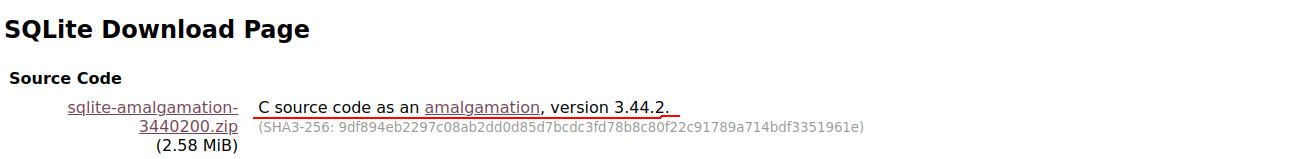
\includegraphics[width=\textwidth]{sqlite.png}
Alternatively, assuming you have wget and you know the version number(in the case 3.44.2), you could also run
\begin{lstlisting}
wget https://www.sqlite.org/2023/sqlite-amalgamation-3440200.zip
\end{lstlisting}

Then unzip the downloaded file.
\subsubsection*{Compiling the CLI interface}
The game uses the command-line interface to generate the game world and the like. To enable the command line, go into the directory
\begin{lstlisting}
gcc shell.c sqlite3.c -lpthread -ldl -lm -o sqlite3
\end{lstlisting}
This 
\section*{Getting,compiling and generating the actual game}
Now that everything has been set up, the time has come to actually get, compile and generate the game world. To do this, simply go in to the revenant/misc folder and run the following shell script
\begin{lstlisting}
./setup_gamle_world.sh
\end{lstlisting}
and then promptly sit back and relax. Chances are, this is going to take a while
\chapter{Source code documentation}
The purpose of this chapter is two-fold
\begin{enumerate}
\item It intends to explain to the player the logic behind how certain things work, for educational purposes.
\item The chapter will also serve as a personal specification / written in stone manual for how certain things are done, to ensure things are done consistently.
\end{enumerate}
\section*{Setup of header files and forward declaration and the db\_reader }
A recurring issue in the code base as coding continued and complexity increased, was the often almost spontaneous discovery of \underline{circular dependencies} - declarations (header files) that would depend on each other:

\begin{center}
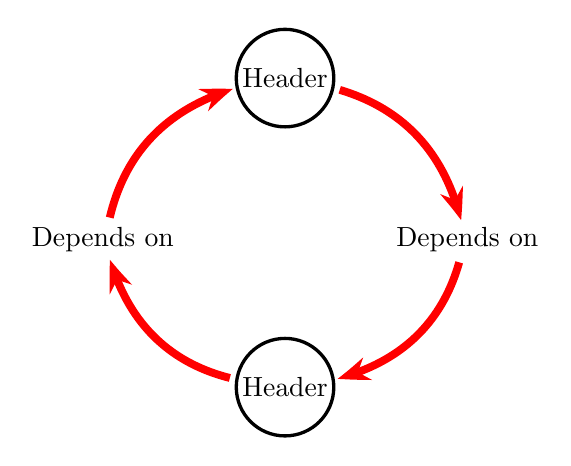
\begin{tikzpicture}[
every node/.append style = {inner sep=1.5pt}, 
node distance = 12mm and 9mm,
 punkt/.style = {circle, draw, very thick},
   pil/.style = {line width=1mm, red, -{Stealth[length=4mm,bend]},
                 shorten >=1pt, shorten <=2pt, bend left=#1},
 pil/.default = 30
                    ]
%nodes
%\node (reward)                                  {$R_t$} ;
\node (state)   [right]               {Depends on} ;
\node (env)     [punkt,
                 below right=of state]          {Header};
\node (action)  [above right=of env]            {Depends on} ;
%
\node (agent)   [punkt, 
                 above=of state.north -| env]   {Header};
% edges
\draw[pil]  (agent)     edge    (action)
            (action)    edge    (env)
            (env)       edge    (state)
%            (env)       edge[pil=40]    (reward)
            (state)     edge    (agent);
%            (reward)    edge[pil=40]    (agent);
\end{tikzpicture}
\end{center}
The solution to this issue was to hyper split the header files in the following manner, containing the following information

\begin{itemize}
\item Struct header files. These would include \textbf{only} struct declarations and constants.
\item "User" header files. These files would in turn define functions and other actual code functionality. Said files would in one way or another make use of the struct header files, hence the classification as users
\end{itemize}

The idea behind this principle is that it would address the primary issue that caused said circular dependencies - namely that functionality in file A would rely on some  functionality in file B that would do some sort of manipulation of structs for file A, that are defined in file A, hence causing said circular dependency:

\begin{center}
\begin{tikzpicture}[
every node/.append style = {inner sep=1.5pt}, 
node distance = 12mm and 9mm,
 punkt/.style = {circle, draw, very thick},
   pil/.style = {line width=1mm, red, -{Stealth[length=4mm,bend]},
                 shorten >=1pt, shorten <=2pt, bend left=#1},
 pil/.default = 30
                    ]
%nodes
%\node (reward)                                  {$R_t$} ;
\node (state)   [right]               {Relies on functionality in ;
\node (env)     [punkt,
                 below right=of state]          {File A};
\node (action)  [above right=of env]            {Depends on} ;
%
\node (agent)   [punkt, 
                 above=of state.north -| env]   {Header};
% edges
\draw[pil]  (agent)     edge    (action)
            (action)    edge    (env)
            (env)       edge    (state)
%            (env)       edge[pil=40]    (reward)
            (state)     edge    (agent);
%            (reward)    edge[pil=40]    (agent);
\end{tikzpicture}
\end{center}

With the new setup (having separate header files for structs and functionality that relies and manipulates structs), this will no longer happen. This is because with the new setup, the "inheritance", going back to the example with the A and B files, will work as follows
\begin{center}
\begin{tikzpicture}[node distance=2.75cm]
%nodes
\node (b_struct) at (4,2)    [draw, circle]   {Struct file B} ;
\node (a_struct)    [draw, circle, below of=b_struct]              {Struct file A} ;
\node (b_user)     [draw, circle, below of=a_struct] {User file B};
\node (a_user)        [draw, circle, below of=b_user]       {User file A};
%edges
\draw [arrow] (b_struct) -- (a_struct);
\draw [arrow] (a_struct) -- (b_user);
\draw [arrow] (b_user) -- (a_user);
\end{tikzpicture}
\end{center}

By separating the definitions of structs and the logic that uses the structs, we have managed to "break" the circular definitions. It is admittedly unknown whether this will cause further headaches down the line, but it succeeds in solving the original issue, which makes it an acceptable solution for now. 

Which brings us to 
\begin{center}
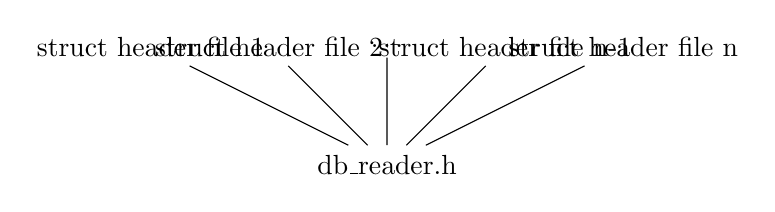
\begin{tikzpicture}[grow'=up]
\node {db\_reader.h}
  child { node {struct header file 1} }
  child { node {struct header file 2} }
  child { node {$\hdots$} }
  child { node {struct header file n-1} }
  child { node {struct header file n} }
;
\end{tikzpicture}
\end{center}

\section*{Naming conventions for the header files}
\subsection*{Naming conventions for the files themselves}
As specified in "Setup of header files and forward declaration and the db\_reader ", there are header files that define only structs and constants and user files, that in some way or another uses said structs. They shall have the name the following name formats
\begin{itemize}
\item Header files that use structs can have whatever name they so desire, as long as they are explanatory
\item Header files, that only define the structs, must end with the \_struct.h, to indicate that it only defines structs and other constants
\end{itemize}
\subsection*{Naming for functions and macros in the files}
Any and all functions/macros, that are defined in the same header file, must begin with the same prefix, e.g if a header file defines 10 functions and the chosen prefix is say, abc, each and every function must begin with abc\_, the prefix should ideally be a descriptive acronym om the intended functionality of the header file.
\section*{Management of game state and status}
\subsection*{Keeping track of the creatures and the player}

\subsection*{Checking for active effects of player}
\subsection*{Creatures}
In the following chapters, we will use several variables to compute various information regarding creatures in-game, their status and the way
that they interact with the environment and the player. For that purpose, we will use the following definitions, some are explicitly computed/stored in-game, others are just definitions and are not explicitly declared in-game. The definitions we will use are
\begin{itemize}
\item $min\_local$ the smallest local coordinate value possible 
\item $max\_local$ the biggest local coordinate value possible 
\item $Player_{global  \:coordinate}$  to represent a player's global coordinate, either X or Y coordinate 
\item $Creature_{global \: coordinate}$ to represent a creature's global coordinate, either X or Y coordinate 
\item The exact same variables are defined for the local coordinates 
\item $max\_moves$ is the maximum number of tiles a player/creature can move, before they move our of bounds of the current screen view. It is computed as  ($max\_local$ - $max\_local$) +1 
\item $Player_{set \: to \: min}$  is a subtraction of the players global coordinate s.t its local coordinate is the minimal. It is computed as  $Player_{global \: coordinate}$ - ($Player_{local \: coordinate}$ - $min\_local$)
\item $Player_{set \: to \: max}$  is an addition of the players global coordinate s.t its local coordinate is the maximal. It is computed as  $Player_{global \: coordinate}$ + ($max\_local$ - $Player_{local \: coordinate}$)
\end{itemize}
With that in mind, we can now go over the different mechanics that we need to consider for the creatures in game, such as spawning, movement, death, behavior, actions and so on

\subsubsection{Spawning creatures}
When it comes to spawning creatures, there are several things that we need to compute in relation to the player. One of them is the creatures local coordinates. The kicker about this is that while a player's local coordinates can be arbitrary without any hassle, the coordinates of the creature must be aligned relative to the players to that the view the creature has on screen matches that of the global coordinates. To do this, there are two cases that need to be considered, the trivial case and the nontrivial case. \newline

In the trivial case, the distance between the player and the creature is s.t the distance for the particular axis, does not exceed the boundaries of the screen \newline

In the non-trivial case, what we effectively do is reduce it to the nontrivial case. The way that we do this is by considering whether the axis-wise coordinate for the player is greater or smaller than the creature's just like in the non-trivial case. In the case that

\[ Player_{global  \:coordinate} > Creature_{global \: coordinate} \]

Then set the creature's local coordinate to
\[ Creature_{local \: coordinate} = max\_local - (Player_{set \: to \: max} - Creature_{global \: coordinate} ) \mod  max\_moves  \]


In the other case where 
\[ Player_{global  \:coordinate} < Creature_{global \: coordinate} \]

Instead, set the creature's local coordinate to

\[ Creature_{local \: coordinate} = min\_local + (Player_{set \: to \: min} - Creature_{global \: coordinate} ) \mod  max\_moves  \]

The workings of this are a little hard to work around. Admittedly, this took rather a long while to figure out and I am unsure whether the computations can get simplified further. However, truth be told, I spent way too long to figure this out and so at this point that I cannot be bothered to come up with more clever solutions. \newline

The way it works (informally) is as follows. Assume that



\section*{Controls}
\subsection*{Keyboard Layout}
This table details all the keyboard bindings for the game. Keyboard bindings with an asterisk indicate that
\begin{table}[h!]
\centering
\begin{tabular}{|c| c| c |c|} 
\hline
 a-m & n-z & A-M & N-Z+ESC \\ [0.5ex] 
 \hline
 a - N/A & n - N/A & A - N/A & N - N/A \\ 
 b - N/A & o - N/A & B - N/A & O - N/A \\
 c - N/A & p - N/A & C - N/A & P - N/A  \\
 d - N/A & q - N/A & D - N/A & Q - N/A  \\
 e - equip item in inventory & r - N/A & E - Show equipped items & R - N/A \\ 
 f - N/A & s - N/A & F - N/A & S - N/A \\
 g - N/A & t - N/A & G - N/A & T - N/A \\
 h - N/A & u - N/A & H - N/A & U - N/A \\
 i - Display current inventory & v - N/A & I - N/A & W - N/A \\
 j - N/A & w - N/A & J - N/A & X- N/A \\
 k - N/A & x - N/A & K - N/A & Y - N/A \\
 l - show past 10 events & y - N/A & L - N/A & Z - N/A \\
 m - N/A & z - N/A & M - N/A & ESC - Quit command \\ [1ex] 
 \hline
\end{tabular}
\caption{Keyboard bindings.}
\label{table:1}
\end{table}




\subsection*{Character meanings on map}
\begin{table}[h!]

\begin{tabular}{|p{0.2\linewidth}|p{0.2\linewidth}| p{0.2\linewidth}|p{0.2\linewidth}|p{0.2\linewidth}|} 
\hline
 a-m & n-z & A-M & N-Z+ESC & Misc. \\ [0.5ex] 
 \hline
 a - animal & n - N/A & A - N/A & N - N/A & @ - player character\\ 
 b - N/A & o - N/A & B - N/A & O - N/A  & ! - interactable npc \\ 
 c - N/A & p - N/A & C - N/A & P - N/A \\
 d - N/A & q - N/A & D - N/A & Q - N/A  \\
 e - N/A & r - N/A & E - N/A & R - N/A \\
 f - N/A & s - N/A & F - N/A & S - N/A \\
 g - N/A & t - trader & G - N/A & T - N/A \\
 h - N/A & u - N/A & H - N/A & U - N/A \\
 i - N/A & v - N/A & I - N/A & W - N/A \\
 j - N/A & w - N/A & J - N/A & X- N/A \\
 k - N/A & x - N/A & K - N/A & Y - N/A \\
 l - N/A & y - N/A & L - N/A & Z - N/A \\
 m - N/A & z - N/A & M - N/A & ESC - Quit command \\ [1ex] 
 \hline
\end{tabular}
\caption{Meaning of characters on screen.}
\label{table:1}
\end{table}
\section*{Interacting with the world}
\subsection*{Dialogue}
\subsubsection*{Dialogue screen and interaction, dialogue-wise}
As unintuitive as it is, dialogue options are \textbf{0-indexed}. This is because it gives a maximum of 10 possible options (0-9), without needing logic for a buffer and instead just accept a single character as player input. As of time of this writing, it is hoped it is never required to have more than 10 options, because it means, as said, we can skimp on buffer logic.

\section*{Managing, reading, writing and manipulation of the game state}
\subsection*{The database}
\subsubsection*{Naming standards}
\paragraph*{Naming standard for variables}
\subparagraph*{Naming of Macros}
Since many values, especially in the context of dialogues are integer id based, and the sqlite interface uses indexes to refer to the values in the columns of the database, the game makes extensive use of macros, to make it clear what it is we are referring to and to reduce the likelihood of errors when index accessing .\newline

Variables that refer to values stored in the columns have two naming formats. This is due to an inconsistency of the sqlite approach for how variables are numbered. When binding variables for queries, the leftmost variable has and index of \textbf{1}, but when retrieving values from a query, the leftmost value has an index of \textbf{0}

Variables that refer column values in the context of a SELECT, UPDATE, DELETE, etc., have the name format of 

\begin{center}
<table name>\_<column name>INDEX\_QUERY
\end{center}

And variables that refer to extracting column values, from a row as a result of a SELECT have the name format of

\begin{center}
<table name>\_<column name>INDEX\_QRESULT
\end{center}

\subparagraph*{Naming conventions for the db\_reader.c \& db\_reader.h files}
All structs, that represent or or more value(s) derived from a query, shall be named *\_Qresult, to indicate it is the result of a query
\subsubsection*{Placement and order of declaration}
\paragraph*{Declaration order for database components}
To ensure readability and ease of information finding, any and all declaration of database objects are made in the misc/ game folder, using shell scripts.

The database objects are to be declared in this order
\begin{enumerate}
\item The table itself
\item Any triggers, indexes, constraints, etc.
\item The values in the table
\end{enumerate}

Each new declaration is to be separated using a dividing line, made from \#\#\#\#\#\#\#\#\#\#\#

At convenience and as needed, each declaration can have elaborating comments
\paragraph*{Declaration order for the db\_reader.c \& db\_reader.h}
By design, the db\_reader functionality will \textit{not} include header information from other revenant components. Instead, any components the need information read in from the DB will include db\_reader in its header files. By doing so, it reduces db\_reader's dependency on the fields contained in the structs of the components that use db\_reader, allowing it to be agnostic wrt. the type and amount of information returned from the queries. 
\chapter*{The world of Revenant}

\section*{Places of Revenant}
\subsection*{Settlements}
\subsubsection*{Iislog}
An incredibly modest 
\section*{Who you are}





















\end{document}
